\begin{frame}{Statistical Error}
    Recall:
    \begin{itemize}
        \item Type I error: rejecting $H_0$ when it is actually true.
        \item Type II error: failing to reject $H_0$ when $H_A$ is actually true.
    \end{itemize}
\end{frame}

\begin{frame}{Adjusting Type II Error}
    We determine how often we commit a Type I error:
    \[
        P(\text{Type I error}) = \alpha
    \]
    but what about Type II errors?
\end{frame}

\begin{frame}{Adjusting Type II Error}
    We can write
    \[
        P(\text{Type II error}) = \beta
    \]
    but what does that tell us?
    
    \vspace{24pt}
    (Note: $\beta$ is the Greek letter "beta".)
\end{frame}

\begin{frame}{Statistical Power}
    \textbf{Power} is the probability that we are able to accurately detect effects.
    \begin{itemize}
        \item This is the \textit{complement} of $\beta$.
        \item There is a trade-off between Type I and Type II error.
        \item We can't set $\beta$ the way we set $\alpha$.
        \item But we know we can decrease Type II error by increasing sample size.
    \end{itemize}
\end{frame}

\begin{frame}{Statistical Power}
    This is another trade-off!
    \begin{itemize}
        \item We want as much data as possible
        \item ...but collecting data can be very expensive.
    \end{itemize}
\end{frame}

\begin{frame}{Power Calculations}
    Goal: determine the sample size necessary to achieve 80\% power.
    
    \vspace{24pt}We will demonstrate using a clinical trial.
\end{frame}

\begin{frame}{Example}
    \begin{itemize}
        \item A company has a new blood pressure drug.
        \item A clinical trial will test its effectiveness.
        \item Study participants are recruited from a population taking a standard blood pressure medication.
        \item Control group: standard medication.
        \item Treatment group: new medication.
    \end{itemize}
\end{frame}

\begin{frame}{Example}
    Write down the hypotheses for a two-sided hypothesis test in this context.
\end{frame}

\begin{frame}{Example}
    \begin{itemize}
        \item Want to run trial on patients with systolic blood pressures b/w 140 and 180 mmHg.
        \item Existing studies suggest:
        \begin{enumerate}
            \item standard deviation of patients’ blood pressures will be about 12 mmHg.
            \item distribution of patient blood pressures will be approximately symmetric.
        \end{enumerate}
    \end{itemize}
    If we had 100 patients per group, what would be the approximate standard error?
\end{frame}

\begin{frame}{Example}
    What does the null distribution of $\bar{x}_{trt} − \bar{x}_{ctrl}$ look like?
    
    \vspace{24pt}
    For what values of $\bar{x}_{trt} − \bar{x}_{ctrl}$ would we reject the null hypothesis?
\end{frame}

\begin{frame}{Example}
    What if we wanted to be able to detect smaller differences?
    
    \vspace{24pt}What if instead we had 200 patients in each group?
\end{frame}

\begin{frame}{Computing Power For Two-Sample Tests}
    \begin{itemize}
        \item We need to determine what is a practically significant result. 
        \item We suppose the researchers care about finding a blood pressure difference of at least 3 mmHgn.
        \item This is called the minimum \textbf{effect size}. 
        \item We want to know how likely we are to detect this size of an effect.
    \end{itemize}
\end{frame}

\begin{frame}{Example}
    \begin{itemize}
        \item Suppose we decide to use 100 patients per treatment group.
        \item The true difference in blood pressure reduction is -3 mmHg.
        \item What is the probability that we are able to reject $H_0$ (given that it's false)?
    \end{itemize}
\end{frame}

\begin{frame}{Example}
    Find the sampling distribution when $\bar{x}_{trt} − \bar{x}_{ctrl} = -3$.
    
    \vspace{24pt}Use this to find the probability that we are able to reject $H_0$ (given that it's false)?
\end{frame}

\begin{frame}{Computing Power For Two-Sample Tests}
    We have a clinical trial with 100 patients in each group and previous studies to suggest a standard deviation of $12$.
    
    \vspace{12pt}
    We want to test
    \begin{itemize}
        \item $H_0:$ $\mu_{trt} - \mu_{trt} = 0$
        \item $H_A:$ $\mu_{trt} - \mu_{trt} \ne 0$
    \end{itemize}
\end{frame}

\begin{frame}{Computing Power For Two-Sample Tests}
    \begin{itemize}
        \item Last class, we found the standard error estimate $SE=1.70$.
        \item This corresponds to rejecting if 
        \[\bar{x}_{trt} − \bar{x}_{ctrl} < -3.33\] 
        or \[\bar{x}_{trt} − \bar{x}_{ctrl} > 3.33\]
    \end{itemize}
\end{frame}

\begin{frame}{Computing Power For Two-Sample Tests}
    Let's redraw the null and sampling distributions for the case where the truth is
    \[
        \mu_{trt} - \mu_{trt} = -3
    \]
\end{frame}

\begin{frame}{Determining Sample Size}
    With a sample size of 100...
    \begin{itemize}
        \item We can only detect an effect size of 3 mmHg with probability 0.42.
        \item This means that the probability of Type II error is 0.58!
        \item For drug development, Type II error could cost a company several hundred million dollars.
    \end{itemize}
\end{frame}

\begin{frame}{Determining Sample Size}
    It is of interest to determine an appropriate sample size. This will allow us to...
    \begin{itemize}
        \item be confident that we are detecting any important effects.
        \item possibly save money in the long-run.
        \item Balance the probability of Type I and Type II error.
    \end{itemize}
\end{frame}

\begin{frame}{Example}
    Suppose now that we recruit 500 patients for each group.
    \begin{itemize}
        \item <1-> Determine the new estimate for standard error.
        \item <2-> Identify the rejection regions.
        \item <3-> Sketch out the null and alternative distributions when $\mu_{trt} - \mu_{trt} = -3$.
        \item <4-> Compute the probability of accurately rejecting $H_0$.
    \end{itemize}
\end{frame}

\begin{frame}{Determining Sample Size}
    We need to find a better balance!
    \begin{itemize}
        \item We can use sample size to find power (we could try a bunch of different numbers)
        \item Or we can flip the problem and use power to find sample size.
        \begin{itemize}
            \item We usually use a power around 80\% or 90\%.
        \end{itemize}
    \end{itemize}
\end{frame}

\begin{frame}{Example}
    What sample size do we need to get a power of 80\%?
    \begin{enumerate}
        \item<1-> Start by assuming normal distribution.
        \begin{itemize}
            \item We will make a correction if later we find $n < 30$.
        \end{itemize}
        \item<2-> Determine the minimum effect size you want to be able to detect.
        \item<3-> Find the Z-score corresponding to a lower tail of 0.80.
    \end{enumerate}
\end{frame}

\begin{frame}{Example}
    \begin{center}
        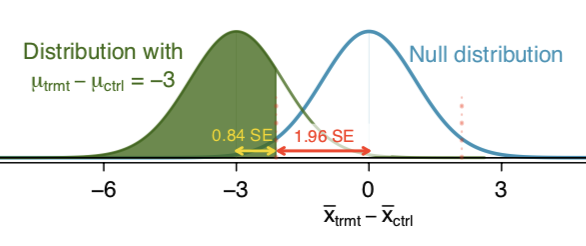
\includegraphics[scale=0.4]{images/nullaltdist.png}
    \end{center}
    \begin{enumerate}\setcounter{enumi}{3}
        \item Find the number of standard deviations between the centers of the two distributions.
    \end{enumerate}
\end{frame}

\begin{frame}{Example}
    \begin{itemize}
        \item The distance between the centers of the two distributions is the minimum effect size of interest.
        \begin{itemize}
            \item we set this when we chose $\mu_{trt} - \mu_{trt} = -3$.
        \end{itemize}
        \item Let's try setting this equal to the distance in standard errors.
        \begin{itemize}
            \item Can we us this to find $n$?
        \end{itemize}
    \end{itemize}
\end{frame}

\begin{frame}{Example}
    Suppose the targeted power was 90\% and we were using $\alpha = 0.01$. 
    
    \begin{enumerate}
        \item How many standard errors should separate the centers of the null and alternative distribution?
        \item What sample size would we need?
    \end{enumerate}
\end{frame}

\begin{frame}{Power Considerations}
    Targeted power will depend on cost:
    \begin{itemize}
        \item Cost to patients (risk).
        \item Cost of enrolling study participants.
        \item Cost of failing to detect an effect of interest.
    \end{itemize}
    If risk and monetary costs are low it makes sense to increase power even if failing to detect an effect of interest isn't a big deal.
\end{frame}

\begin{frame}{Power Considerations}
    However...
    \begin{center}
        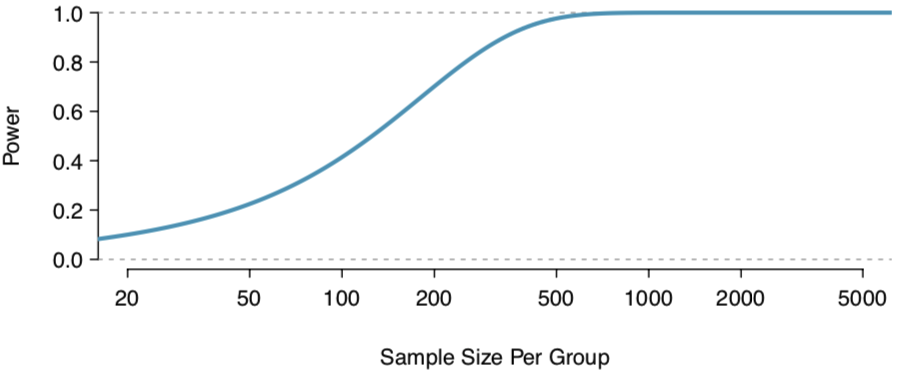
\includegraphics[scale=0.3]{images/pwrplot.png}
    \end{center}
    there's often a ceiling!
\end{frame}

\begin{frame}{Example}
    A large farm wants to try out a new type of fertilizer to evaluate whether it will improve the farm's corn production. The land is broken into plots that produce an average of 1215 pounds of corn with a standard deviation of 94 pounds per plot. The owner is interested in detecting any average difference of at least 40 pounds per plot. How many plots of land would be needed for the experiment if the desired power level is 90\%? Assume each plot of land gets treated with either the current fertilizer or the new fertilizer.
\end{frame}
